 %\chapter{Background}
\section{Background \& Theoretical Basics }

In this chapter, we provide high-level explanations of the most important aspects and comprehensive understanding of the foundational theories and principles that make query optimization and materialized views effective. The concrete basics needed are explained the respective section along the thesis.

%some basics of the Database particularly distributed database.Then an overview of materialized view as query processing technique. later,we will discuss various methods and algorithms to about materialized view and Finally we discuss related work.
\subsection{ Database System}

\begin{definition}
A database is an organized collection of data or a type of data store based on the use of a database management system(DBMS), the software that enables the creation, modification and the database itself to capture and analyze the data.\end{definition}\vspace{.4cm}
A database in SQL Server is made up of a collection of tables that stores a specific set of structured data. A table contains a collection of rows, also refereed to as records or tuples and columns also referred to as attributes. Each column in the table is designed to store a certain type of information, for example: dates, names, dollar and numbers.\cite{williamdassafmsft-2024} Scalability, security, high availability, Network latency, fault tolerance these are the key characteristics of databases. There are two most distinct types of databases: Relational and NoSQL database.

\begin{itemize}
    \item \textbf{Relational databases(RDBMS) :} The relational database model came about 1969-70 as a solution for dealing with the variety of custom designed DBMSs that were used, prior to 1969. These databases store the data in structured tables with rows and columns and use for SQL for querying. They are known for their robustness, flexibility, and support for ACID properties. Example: Microsoft SQL server, MySQL, PostgreSQL, Oracle database.\cite{editor-2024,foote-2023}
    
    \item \textbf{NoSQL databases:} NoSQL, also referred to as "not only SQL", emerged in the late 2000s, is an approach to database design that enables the storage and querying of data outside the traditional structures found in relational database. It offers flexibility and scalability, making them particularly useful for handling large amounts of unstructured data in real time applications. They support horizontal scaling allowing for increased storage and processing capabilities as data volume grow. Example: MongoDB, Redis, CouchDB.\cite{ibm-2024,justacademy_nosql_characteristics}
\end{itemize}

\subsection{Query Processing }
A query is a request sent to a database for data retrieval. Specific conditions are passed in a query to match and retrieve relevant data. SQL (Structured Query Language) is used to write these queries to extract information from relational databases. The query process involves translating high-level queries into low-level expressions suitable for the file system, optimizing the query, and executing it to obtain the result. The steps involved in the execution of a query are as follows:\cite{wwwnaukricom-no-date}\\
\begin{figure}[h]
    \centering
    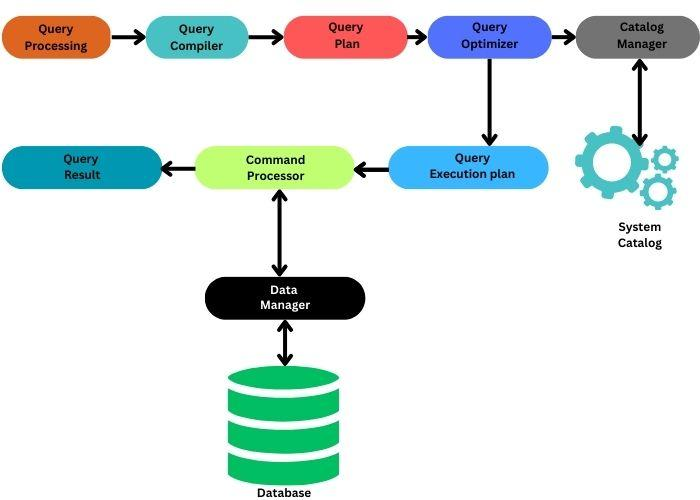
\includegraphics[width=0.5\textwidth]{Figure/Flow of QueryProcessing.jpg}
    \caption{The flow of query processing in DBMS.}
    \label{fig:my_image}
\end{figure}
\begin{enumerate}
\item \textbf{Parser:} Query parsing is the first step in query processing. In this steps, database performs the following checks- Syntax,semantic and shared pool check,after converting the query into relational algebra.\cite{wwwnaukricom-no-date}
    \begin{enumerate}
        \item \textbf{Syntax check:} A query is checked for syntax error.It concludes syntactic validity. Example:\\
        % Define colors
\definecolor{codegreen}{rgb}{0,0.6,0}  % Green for comments
\definecolor{codegray}{rgb}{0.5,0.5,0.5}  % Gray for numbers
\definecolor{codepurple}{rgb}{0.58,0,0.82}  % Purple for strings
\definecolor{backcolour}{rgb}{0.95,0.95,0.92}  % Light gray background
\definecolor{bordercolor}{rgb}{0.7,0.7,0.7}  % Left border color (gray)
\definecolor{codeblue}{rgb}{0,0,0.8}  % Blue for SQL keywords

\lstdefinelanguage{MySQL}{
    keywords={SELECT, FROM, WHERE, JOIN, ON, INNER, OUTER, LEFT, RIGHT, FULL, GROUP, BY, ORDER, ASC, DESC, AS, COUNT, SUM, AVG, MAX, MIN, DISTINCT, INSERT, INTO, VALUES, UPDATE, SET, DELETE, CREATE, TABLE, PRIMARY, FOREIGN, KEY, DEFAULT, NULL, NOT, CHECK, CONSTRAINT, INDEX, VIEW, MATERIALIZED, PROCEDURE, FUNCTION, TRIGGER, DATABASE, ALTER, DROP, EXEC, IF, EXISTS, UNION, ALL, CASE, WHEN, THEN, ELSE, END, CAST, CONVERT, LIKE, IN, BETWEEN, AND, OR, HAVING, LIMIT, OFFSET},
    sensitive=false,
    morestring=[b]',  % String in single quotes
    morestring=[b]"   % String in double quotes
}
\captionsetup[lstlisting]{font=small}
\lstdefinestyle{sqlstyle}{
    backgroundcolor=\color{backcolour},   
    commentstyle=\color{codegreen},  % Comments in green
    keywordstyle=\bfseries\color{codeblue},  % ✅ SQL Keywords in Blue & Bold
    numberstyle=\scriptsize\color{codegray},  % Row numbers in gray
    stringstyle=\color{codepurple},  % Strings in purple
    basicstyle=\ttfamily\footnotesize,
    breaklines=true,
    captionpos=b,
    numbers=left,      % ✅ Enables row numbers on the left
    stepnumber=1,      % ✅ Row numbers increment by 1
    firstnumber=1,     % ✅ Starts numbering at 1
    numbersep=8pt,     % ✅ Increases space between numbers and SQL code
    xleftmargin=3em,   % ✅ Ensures space inside the left border
    frame=single,      % ✅ Keeps a single border (left-aligned)
    framesep=5pt,      % ✅ Ensures space inside the frame
    rulesepcolor=\color{bordercolor},  % ✅ Matches row numbers with left border
    rulecolor=\color{bordercolor},  % ✅ Sets left border color
    language=MySQL  % ✅ Uses SQL keyword highlighting
}



\begin{lstlisting}[style=sqlstyle, caption={SQL query to check syntax}]
SQL>SELECT * form employees;SELECT * form employees * error at line 1:
FROM   keyword NOT found
WHERE  expected
\end{lstlisting}
          Here error of wrong spelling of FROM is given by this check.
        \item \textbf{Semantic check:} It checks whether the statement is meaningful or not. Example: Query contains a table name which doesn't exist\\
        
\definecolor{dkgreen}{rgb}{0,0.6,0}
\definecolor{gray}{rgb}{0.5,0.5,0.5}
\definecolor{mauve}{rgb}{0.58,0,0.82}
\lstset{language=SQL,
  basicstyle={\small\ttfamily},
  belowskip=3mm,
  breakatwhitespace=true,
  breaklines=true,
  classoffset=0,
  columns=flexible,
  commentstyle=\color{dkgreen},
  framexleftmargin=0.25em,
  frameshape={}{yy}{}{}, %To remove to vertical lines on left, set `frameshape={}{}{}{}`
  keywordstyle=\color{blue},
  numbers=none, %If you want line numbers, set `numbers=left`
  numberstyle=\tiny\color{gray},
  showstringspaces=false,
  stringstyle=\color{mauve},
  tabsize=3,
  xleftmargin =1em
}
         \begin{lstlisting}
         SQL> SELECT * FROM nonexistent_table;
         SELECT * FROM nonexistent_table
              *
        ERROR at line 1:
        ORA-00942: table or view does not exist
        FROM keyword not found where expected
        \end{lstlisting}
        A syntactically correct statement can fail a semantic check, as shown in the following example of a query of a nonexistent table.\cite{Oracle}
        \item \textbf{Shared pool check:} During the parse, the database performs a shared pool check to determine whether it can skip (hash code )resource-intensive steps of statement processing. Every query posses a hash code..
        % Define colors
\definecolor{codegreen}{rgb}{0,0.6,0}  % Green for comments
\definecolor{codegray}{rgb}{0.5,0.5,0.5}  % Gray for numbers
\definecolor{codepurple}{rgb}{0.58,0,0.82}  % Purple for strings
\definecolor{backcolour}{rgb}{0.95,0.95,0.92}  % Light gray background
\definecolor{bordercolor}{rgb}{0.7,0.7,0.7}  % Left border color (gray)
\definecolor{codeblue}{rgb}{0,0,0.8}  % Blue for SQL keywords

\lstdefinelanguage{MySQL}{
    keywords={SELECT, FROM, WHERE, JOIN, ON, INNER, OUTER, LEFT, RIGHT, FULL, GROUP, BY, ORDER, ASC, DESC, AS, COUNT, SUM, AVG, MAX, MIN, DISTINCT, INSERT, INTO, VALUES, UPDATE, SET, DELETE, CREATE, TABLE, PRIMARY, FOREIGN, KEY, DEFAULT, NULL, NOT, CHECK, CONSTRAINT, INDEX, VIEW, MATERIALIZED, PROCEDURE, FUNCTION, TRIGGER, DATABASE, ALTER, DROP, EXEC, IF, EXISTS, UNION, ALL, CASE, WHEN, THEN, ELSE, END, CAST, CONVERT, LIKE, IN, BETWEEN, AND, OR, HAVING, LIMIT, OFFSET},
    sensitive=false,
    morestring=[b]',  % String in single quotes
    morestring=[b]"   % String in double quotes
}

\lstdefinestyle{sqlstyle}{
    backgroundcolor=\color{backcolour},   
    commentstyle=\color{codegreen},  % Comments in green
    keywordstyle=\bfseries\color{codeblue},  % ✅ SQL Keywords in Blue & Bold
    numberstyle=\scriptsize\color{codegray},  % Row numbers in gray
    stringstyle=\color{codepurple},  % Strings in purple
    basicstyle=\ttfamily\footnotesize,
    breaklines=true,
    captionpos=b,
    numbers=left,      % ✅ Enables row numbers on the left
    stepnumber=1,      % ✅ Row numbers increment by 1
    firstnumber=1,     % ✅ Starts numbering at 1
    numbersep=8pt,     % ✅ Increases space between numbers and SQL code
    xleftmargin=3em,   % ✅ Ensures space inside the left border
    frame=single,      % ✅ Keeps a single border (left-aligned)
    framesep=5pt,      % ✅ Ensures space inside the frame
    rulesepcolor=\color{bordercolor},  % ✅ Matches row numbers with left border
    rulecolor=\color{bordercolor},  % ✅ Sets left border color
    language=MySQL  % ✅ Uses SQL keyword highlighting
}



\begin{lstlisting}[style=sqlstyle, caption={SQL query to check shared pool}]
     ALTER SESSION SET OPTIMIZER_MODE=ALL_ROWS;
     ALTER SYSTEM FLUSH SHARED_POOL; 
     SELECT * FROM Employees WHERE DepartmentID = 10;

\end{lstlisting}
        In this example, the same \textbf{SELECT} statement is executed in three different optimizer environments. As a result database creates three separate shared SQL areas for these statements and force a hard parse of each statement.\cite{Oracle}
    \end{enumerate}.\\
\begin{figure}[h]
    \centering
    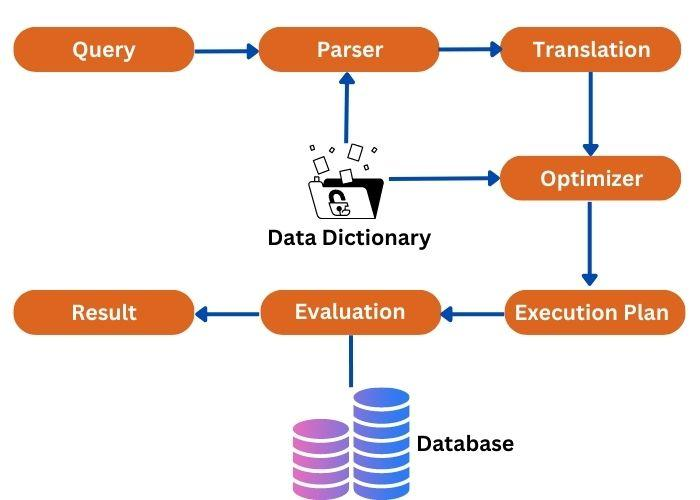
\includegraphics[width=0.5\textwidth]{Figure/Query processing.jpg}
    \caption{The flow of query processing in DBMS}
    \label{fig:my_image}
\end{figure}
    
    \item \textbf{Optimizer}: After parsing the query, the DBMS starts to find the most efficient way of executing the provided query. The factors for the query follow some optimization process. During the optimization stage, at least one complex parsing of one unique DML statement must be done. The database never optimizes DDL unless it includes a DML component, such as a sub-query, which needs optimization. Such operations are used for selecting data, inserting something, updating, etc. After everything is completed, then the evaluation step is made. in this step, the result is returned by the DBMS. This result is displayed to you in an appropriate format.
    \item \textbf{Result:} After getting the best execution plan, the DBMS starts the execution of the optimized query and perform the operation on data including selecting the data, inserting something, updating the data.\\
    Once everything is completed, DBMS returns the result after the evaluation step. This result is shown to you in a suitable format.\cite{Query,QueryProcessing,Oracle}
\end{enumerate}

\subsection{Query Optimization }When we write code, we aim for optimal logic in terms of both space and time complexity. Similarly, when we write database queries, we want them to be optimal in terms of their execution time and resource utilization's. Query optimization is  a crucial aspect of DBMS that seeks the most efficient way to execute a given query by considering a variety of query execution strategies. It minimizing the total cost or the total response time for the execution of a query.It is one of the factors that affect the application performance.\vspace{.4cm}

The result of a query is generated by processing the rows in a database in a way that yields the requested information. Since database structure are complex,in most cases and especially for not very simple queries, the needed data for a query can be collected from a database by accessing it  in different ways through different data structure and in different orders\cite{selinger-1979}. Each different way typically requires different processing time. Processing time of the same query may have large variance, from a fraction of a second to hours, depending on the chosen method. The purpose of a query optimization is to find the way to process a given query in minimum time, the large possible variance in time justifies performing query optimization, though finding the exact optimal query plan among all possibilities, is typically very complex, time consuming by itself may be too costly, and often practically impossible. Thus query optimization typically tries to approximate the optimum by comparing several common-sense alternatives to provide in a reasonable time.\vspace{.4cm}

There is a trade off between the amount of time spent figuring out the best query plan and the quality of the choice, the optimizer may not choose the best answer on its own. Different qualities of database management systems have different ways of balancing these two. Cost based query optimizes  evaluate the resource footprints of various query plans and use this as the basis for plan selection.These assign an estimated cost to each possible query plan and choose the plan with the smallest cost. Cost are used to estimate the runtime cost of evaluating the query, in terms of number of I/O operations required, cpu path length, amount of disk buffer space, disk storage service time, and interconnect usage between units of parallelism and other factors determined from the data directory. The set of query plans examined is formed by examining the possible access paths e.g. primary index, secondary index access, full file scan and various relational table join techniques e.g Merge join, Has join, Product join. the search space can become  quite large depending on the complexity of the SQL query. There are two types of optimization. These consist of logical optimization-which generates a sequence of relational algebra to solve the query-and physical optimization-which is used to determine the means of carrying out each operation.\cite{dremio-2024}


\subsubsection{Database query performance Metrics}
To effectively measure the performance of SQL queries, the following metrics are playing vital role. But most relevant metrics may vary depending on the specific database system and application requirements.
Here is a summery of key metrics used to evaluate and enhance query performance.\cite{chwesewicz-2024}
\begin{itemize}
    \item\textbf{Query execution time}: Total query duration to execute from start to finish. Measured in seconds or milliseconds. Lower execution time indicates better performance.
    \item\textbf{Query throughput}: It measures the number of queries or operation a database can handle per unit time, typically expressed as transaction per second (TPS) and queries per second(QPS).
    \item\textbf{Resource utilization}: Measures the percentage of time the CPU is occupied processing database operations. High CPU or memory usages can indicate heavy processing load or un-optimized queries.
\end{itemize}
\subsubsection{Key optimization techniques:}
 \begin{itemize}
     \item \textbf{Indexing}: Indexing is a crucial technique for query optimization in databases. It's named indexing because of how an index works in a book. An index is a structure that holds the field the index is sorting and a pointer from each record to their corresponding record in the original table where data is actually stored.\cite{tomar-2021,atlassian-no-date}
     \item \textbf{Query rewriting}: It is a technique that used in query optimization to transform a given database query into an equivalent form that executes more efficiently. It is one of the initial phases of query processing where original query is parsed and translated into an internal representation. This method particularly useful for complex queries, including those queries that have many sub queries or many joins.\cite{pitoura-2009,unknown-IBM-25-2024}
     \item \textbf{Partitioning}: This optimization method is specially  effective for large database. It involves splitting a large table or index into smaller segments to make the query more manageable pieces. Each partition acts as a separate entity that can be managed independently.\cite{planck-2024} 
     \item \textbf{Materialized view}: Materialized views are a powerful tool for query optimization, which we will focus on. 
 \end{itemize}
 
 \subsection{Reasons for Using Materialized Views for Query Optimization}:
\begin{itemize}
    \item\textbf{Precomputed result:} Materialized views store the results of a query that allows subsequent queries to access these precomputed results directly rather than recalculating them from the base tables. These results are updated periodically or on demand based on the underlying data changes.\cite{khan-2023,Risingwave-no-date}
    \item\textbf{Reduced Query complexity:} The main reason for creating materialized views is to improve query performance. It stores a snapshot of the data, that reduces the need for intricate query design, as we get the accesses precomputed results directly.\cite{Risingwave-no-date,Databricks-no-date}
    \item\textbf{Efficient use of resources:} As we  get the data from precomputed data and don't need to run full query every time materialized views decrease the computational load on database servers. It leads faster query response time and improved overall system performance and required fewer resources.\cite{google-no-date, khan-2023}
    
\end{itemize}\vspace{.4cm}

The motivation for using materialized views is to improve performance but the overhead associated with materialized view management can become a significant system management problem. The common materialized view management activities include: identifying which materialized view to create, indexing the materialized view; ensuring that all materialized views and materialized view indexes are refreshed properly each time the database is updated; checking which materialized views have been used; determining how effective each materialized view has been on workload performance; measuring the space being used by materialized views; determining which existing materialized views should be dropped,  archiving old detail and materialized view data that is no longer useful.\cite{Ashadevi2008CostEA,1363763}

\subsubsection{Challenges in query optimization} Query optimization is a crucial aspect of database management, aiming to improve the performance and efficiency of SQL queries.
\begin{itemize}
    \item\textbf{Data Fragmentation and Localization}: Dealing with how data is partitioned and distributed across multiple nodes. Data can be fragmented both horizontally and vertically and spread across nodes. Balancing between local execution and data transfer is also challenging. 
    \item\textbf{Query Decomposition and Allocation}: It refers to the process of breaking down a query into sub queries and assign them to different nodes.Challenging to choose best sub queries and node.
    \item\textbf{Complexity of Query Execution Plans}: Query optimization involves various techniques. Mastering these techniques can be challenging to find the most efficient one, especially for complex or multi-table queries.
    \item\textbf{Dependency on Indexes}: Proper indexing improves query performance but failing to create or maintain supporting indexes can result in inefficient query executions. Managing and updating indexes as data grows and changes can become a challenge.\\
    \cite{team-2020,etutorials-03-2024,editor-ijmter-2015}
\end{itemize}
\subsubsection*{Optimization Goals:}

\begin{itemize}
    \item Minimize response time
    \item Minimize resource consumption
    \item Minimize time to first tuple
    \item Maximize throughput
\end{itemize}\vspace{.4cm}

Expressed during optimization as a cost function. The common choice is to minimize response time within given resource limitations.



\subsection{What is a view in SQL:}
Views are perspective on a database. A view provides data of a database to a client and simultaneously prevents client access to the original database tables. When discussing views, the database tables always referred to as the view tables. View tables can reproduce the data of a database, they can provide a specific selection of data or they can compute new data out of the base table contents. Basically any analytical operation that can be derived from base table data can also be represented in a view table.\vspace{.4cm}

A view in SQL is a a virtual table that is generated by an SQL query. It does not store data physically but retrieves it from the underlying base table.Views are compiled at runtime, and they simplify the presentation of data from one or more tables without modifying the original data. It can be made over one or more database tables. Generally, we put those column in view that we need to query again and again. Once we created a view, we can make index, trigger on the view and query the view as table. A view may act as a filter on certain tables being referenced in the view \cite{chauhan-2024,Rohan_Vats-2024}

\subsubsection{Types of Views:}

There are two types of view in SQL server
\begin{itemize}
    \item \textbf{System defined view }: The system defined views are predefined views that already exists in the  master database of SQL server, such as tempdb, master and temp. Each of the database has its own properties and function. These system views will be automatically attached to any user-defined database.It will expose the metadata of the database and they can be used to get all possible information about the instance of SQL server or database objects, columns and contains. There are three types of System defined views, Information Schema, Catalog View, and Dynamic Management View. \cite{chauhan-2024}
    \item \textbf{User defined view }: This are the types of views that are defined by the user. User defined these view to meet their specific requirements.It can also divide into three types such as simple,complex and materialized views.\cite{javapoint-author-2024}
\end{itemize}
   
